\documentclass[conference]{IEEEtran}
\IEEEoverridecommandlockouts
% The preceding line is only needed to identify funding in the first footnote. If that is unneeded, please comment it out.
\usepackage{cite}
\usepackage{amsmath,amssymb,amsfonts}
\usepackage{algorithm}
\usepackage{algorithmic}
\usepackage{graphicx}
\usepackage{textcomp}
\usepackage{xcolor}
\DeclareMathOperator*{\argmin}{arg\,min}
\def\BibTeX{{\rm B\kern-.05em{\sc i\kern-.025em b}\kern-.08em
    T\kern-.1667em\lower.7ex\hbox{E}\kern-.125emX}}
\begin{document}

\title{Infinite-Horizon Stochastic Optimal Control\\
}

\author{\IEEEauthorblockN{Awies Mohammad Mulla}
\IEEEauthorblockA{amulla@ucsd.edu}}

\maketitle



\section{Introduction} \label{sec:intro}
In this project, we are attempting to design a controller which can effectively track and follow a reference trajectory for a ground differential-drive robot.
The controller should be able to handle disturbances and uncertainties in the system. The controller should also be able to avoid the collision.
This because the given trajectory is not collision free. Ideally, in robotics we first solve the motion planning problem where we take care of the collision
such that the reference trajectory is always collision free. But even then the controller should be designed to handle the collisions. 
This is because controller provides us with the values such that the agent follows follows a smooth trajectory due to the 
constraints present in the actuators. So, it might hit the obstacles even though the reference trajectory is collision free.
The reference trajectory along with the result of simple proportional controller is shown in the Figure \ref{fig:reference_trajectory}.
\begin{figure}[h]
    \centering
    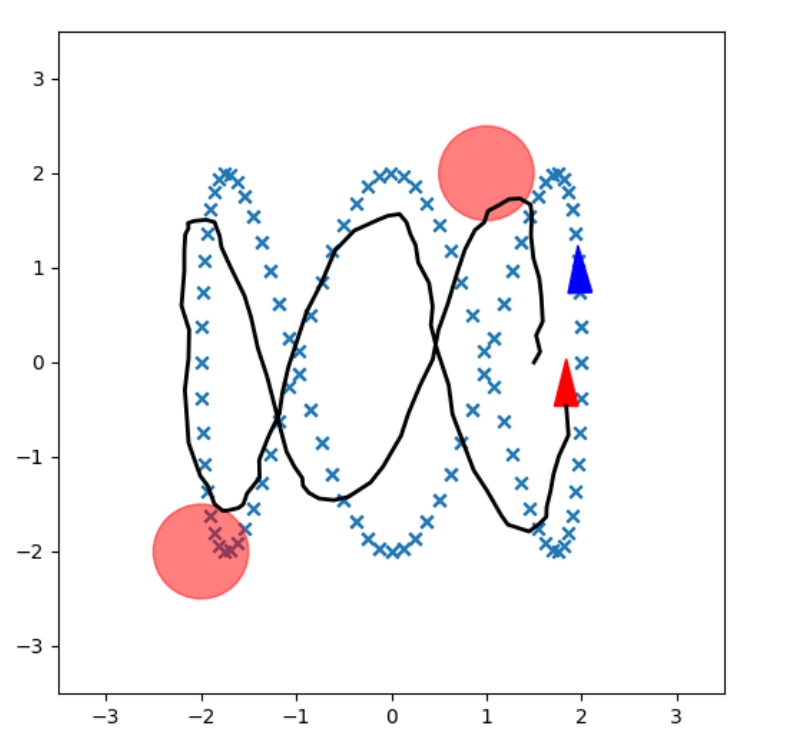
\includegraphics[width=0.5\textwidth]{intro.png}
    \caption{Reference shown in blue and the trajectory followed by the agent shown in black.}
    \label{fig:reference_trajectory}
\end{figure}
The system is also subjected to simulated gaussian noise. We will tackling this problem by formulating a
infinite-horizon stochastic optimal problem. The problem is solved using two approaches. In both the approaches our goal is to minimze the 
cost function which is function of the error between the reference trajectory and the trajectory followed by the agent according to the calculated control input.

The first approach is to design a receding-horizon Certainty Equivalent Control (CEC). In this approach we would assume that the system is assumed to be deterministic
and we iteratively solving a discounted finite-horizon optimal control problem. We can assume that the system is deterministic 
because the controller solves the finite-horizon optimal control problem iteratively upto a particular horizon length. Hence, it is 
because of this online re-planning CEC formulation can afford to assume that the system is deterministic. The implementation of this approach is 
almost identical to the well-known Model Predictive Control (MPC) approach. The only difference is that in MPC we solve the finite-horizon optimal control problem
with respect to the state of the system, whereas here we have formulated our problem around the error between the reference trajectory and the trajectory followed by the agent.
We would design the constraints of our optimization problem such that agent avoids the obstacles and the control input is within the limits of the actuators.

The second approach is Generalized Policy Iteration Algorithm. In this approach we would directly solve the original infinite-horizon stochastic optimal control problem.
using policy iteration algorithm. Since, the dynamics of the system is continuous, to implement the policy iteration 
algorithm we would have to discretize the state and the control appropriately. This is one the major difference in both the approaches. Although 
the problem of obstacle avoidance is quite straightforward, the problem arises while discretizing the state and the control. This is because a
controller should be fast enough to avoid any dynamic changes in the environment in real-time. And increasing the resolution of the discretization 
would largely increase the computation time. Hence, we would have to find a trade-off between the computation time and the resolution of the discretization.

\section{Problem Formulation}
The state of the system is given by $\mathbf{x}_t = (\mathbf{p}_t, \theta_t)$, where $\mathbf{p}_t \in \mathbb{R}^2$ is the position of the agent at discrete time $t$ and $\theta_t \in [-\pi, \pi)$ is the orientation of the agent at time $t$.
The robot is controlled by the control input $\mathbf{u}_t = (v_t, \omega_t)$, where $v_t \in \mathbb{R}$ is the linear velocity and $\omega_t \in \mathbb{R}$ is the angular velocity (yaw rate) of the robot at time $t$.
The discrete-time kinematic model of the differential-drive robot obtained from Euler discretization of the continuous-time kinematic model with time interval $\Delta > 0$ is given by
\begin{align}\label{eq:kinematic_model}
    \mathbf{x}_{t+1} &= \begin{bmatrix}
        \mathbf{p}_{t+1} \\ \theta_{t+1}
    \end{bmatrix} = f(\mathbf{x}_t, \mathbf{u}_t, \mathbf{w}_t) \\
    &= \begin{bmatrix}
        \mathbf{p}_t \\ \theta_t \end{bmatrix} + \begin{bmatrix}
            \Delta \cos(\theta_t) & 0 \\ \Delta \sin(\theta_t) & 0 \\ 0 & \Delta
        \end{bmatrix} \begin{bmatrix}
            v_t \\ \omega_t
        \end{bmatrix} + \mathbf{w}_t \\
    &=  \mathbf{x}_t + \mathbf{G}(\mathbf{x}_t) \mathbf{u}_t + \mathbf{w}_t,
\end{align}
where $\mathbf{w}_t \in \mathbb{R}^3$ models the motion noise with Gaussian distribution $\mathcal{N}(\mathbf{0}, \text{diag}(\mathbf{\sigma})^2)$  with standard deviation $\mathbf{\sigma} = (0.04, 0.04, 0.004)$.
The control input $\mathbf{u}_t$ is constrained by the actuator limits $\mathcal{U} = [0,1] \times [-1, 1]$ for linear and angular velocity, respectively. Since, the reference 
trajectory is present in a finite cartesian space, we would define the configuration space of the agent as $ \mathcal{F} = [-3, 3]^2 \backslash (\mathcal{C}_1 \cup \mathcal{C}_2)$, where $\mathcal{C}_1$ and $\mathcal{C}_2$ are the circles of radius $0.5$ centered at $(-2, -2)$ and $(1, 2)$, respectively acting as the obstacle.
The reference position trajectory is given by $\mathbb{r}_t \in \mathbb{R}^2$ and the reference orientation trajectory is given by $\alpha_t \in [-\pi, \pi)$.

As mentioned in \ref{sec:intro}, we would mostly be working the error between the reference trajectory and the trajectory followed by the agent. Hence, we would define the error state as $\mathbf{e}_t = (\bar{\mathbf{p}}_t, \bar{\theta}_t)$, where $\bar{\mathbf{p}}_t = \mathbf{p}_t - \mathbf{r}_t$ and $\bar{\theta}_t = \theta_t - \alpha_t$
measure the poistion and orientation deviation from the reference trajectory, respectively. The equations for motion of the error state are:
\begin{align}\label{eq:error_model}
    \mathbf{e}_{t+1} &= \begin{bmatrix}
        \bar{\mathbf{p}}_{t+1} \\ \bar{\theta}_{t+1}
    \end{bmatrix} = g(t, \mathbf{e}_t, \mathbf{u}_t, \mathbf{w}_t) \\
    &= \begin{bmatrix}
        \bar{\mathbf{p}}_t \\ \bar{\theta}_t \end{bmatrix} + \begin{bmatrix}
            \Delta \cos(\bar{\theta}_t + \alpha_t) & 0 \\ \Delta \sin(\bar{\theta}_t + \alpha_t) & 0 \\ 0 & \Delta
        \end{bmatrix} \begin{bmatrix}
            v_t \\ \omega_t
        \end{bmatrix} + \begin{bmatrix}
            \mathbf{r}_t - \mathbf{r}_{t+1} \\ \alpha_t - \alpha_{t+1}
        \end{bmatrix} + \mathbf{w}_t \\
    &=  \mathbf{e}_t + \tilde{\mathbf{G}}(\mathbf{e}_t) \mathbf{u}_t + \begin{bmatrix}
            \mathbf{r}_t - \mathbf{r}_{t+1} \\ \alpha_t - \alpha_{t+1}
        \end{bmatrix} + \mathbf{w}_t
\end{align}
\subsection{General Policy Iteration Algorithm}
We formulate the trajectory tracking problem with initial time $\tau$ and initial tracking error $\mathbf{e}_\tau$ as an infinite-horizon stochastic optimal control problem:
\begin{align}\label{GPI}
    \pi^*(\tau, \mathbf{e}_\tau) &= \argmin_{\pi} \mathbb{E} \left[ \sum_{t=\tau}^\infty \gamma^{t-\tau} \ell(\mathbf{e}_t, \mathbf{u}_t) | \mathbf{e}_{\tau} = \mathbf{e} \right] \\
    \text{s.t.} \quad \mathbf{e}_{t+1} &= g(t, \mathbf{e}_t, \mathbf{u}_t, \mathbf{w}_t) \\
    \mathbf{u}_t &\in \mathcal{U} \\
    \mathbf{w}_t &\sim \mathcal{N}(\mathbf{0}, \text{diag}(\mathbf{\sigma})^2) \\
    \bar{\mathbf{p}_t} + \mathbf{r}_t &\in \mathcal{F} \\
    t &= \tau, \tau+1, \dots
\end{align}
where, $\gamma \in (0, 1)$ is the discount factor and $\ell(\mathbf{e}_t, \mathbf{u}_t)$ is the stage cost. The optimal policy $\pi^*$ is a mapping from the initial tracking error $\mathbf{e}_\tau$ to the optimal control sequence $\mathbf{u}_\tau^*, \mathbf{u}_{\tau+1}^*, \dots$.
The stage cost is defined as
\begin{equation}
    \ell(\mathbf{e}_t, \mathbf{u}_t) = \bar{\mathbf{p}_t}^{T} \mathbf{Q} \bar{\mathbf{p}_t} + q(1 -\cos(\bar{\theta}_t))^2 + \mathbf{u}_t^T \mathbf{R} \mathbf{u}_t
\end{equation}
where, $\mathbf{Q} \in \mathbb{R}^{2 \times 2}$, $\mathbf{R} \in \mathbb{R}^{2 \times 2}$ and $q \in \mathbb{R}$ are the positive definite matrices and scalar, respectively. The matrices $\mathbf{Q}$ and $\mathbf{R}$ are the matrices penalizing the deviation from the reference position trajectory $\mathbf{r}_t$ and the control $\mathbf{u}_t$, respectively. The scalar $q$ is the weight for the orientation error. The optimal policy $\pi^*$ is a mapping from the initial tracking error $\mathbf{e}_\tau$ to the optimal control sequence $\mathbf{u}_\tau^*, \mathbf{u}_{\tau+1}^*, \dots$.
\subsection{Certainty Equivalent Control} \label{sec:ce}
As mentioned in \ref{sec:intro}, we would be using the certainty equivalent control approximates the infinite-horizon problem by repeatedly solving a finite-horizon deterministic optimal control problem at each time step:
\begin{align}
    \pi^*(\tau, \mathbf{e}_\tau) &= \argmin_{\pi} \mathbf{q}(\mathbf{e}_{\tau + N}) + \sum_{t=\tau}^{\tau+N-1} \gamma^{t-\tau} \ell(\mathbf{e}_t, \mathbf{u}_t) \\
    \text{s.t.} \quad \mathbf{e}_{t+1} &= g(t, \mathbf{e}_t, \mathbf{u}_t, 0) \\
    \mathbf{u}_t &\in \mathcal{U} \\
    \bar{\mathbf{p}_t} + \mathbf{r}_t &\in \mathcal{F} \\
    t &= \tau, \tau+1, \dots, \tau+N-1
\end{align}
where, $\mathbf{q}(\mathbf{e}_{\tau + T})$ is the terminal cost to be chosen, $N$ is the horizon length to be decided and $\ell(\mathbf{e}_t, \mathbf{u}_t)$ is the stage cost given by
\begin{equation}
    \ell(\mathbf{e}_t, \mathbf{u}_t) = \bar{\mathbf{p}_t}^{T} \mathbf{Q} \bar{\mathbf{p}_t} + q(1 -\cos(\bar{\theta}_t))^2 + \mathbf{u}_t^T \mathbf{R} \mathbf{u}_t
\end{equation}
The receding-horizon CEC problem is now a non-linear program (NLP) program of the form:
\begin{align}
    & \min_{\mathbf{U}} c(\mathbf{U}, \mathbf{E}) \\
    & \text{s.t.} \quad \mathbf{U}_{lb} \leq \mathbf{U} \leq \mathbf{U}_{ub} \\
    & \mathbf{h}_{lb} \leq \mathbf{h}(\mathbf{U}, \mathbf{E}) \leq \mathbf{h}_{ub}
\end{align}
where, $\mathbf{U} = [\mathbf{u}_\tau^T, \mathbf{u}_{\tau+1}^T, \dots, \mathbf{u}_{\tau+N-1}^T]^T$ is the decision variable, $\mathbf{E} = [\mathbf{e}_\tau^T, \mathbf{e}_{\tau+1}^T, \dots, \mathbf{e}_{\tau+N}^T]^T$ is the state variable, $c(\mathbf{U}, \mathbf{E})$ is the cost function, $\mathbf{h}(\mathbf{U}, \mathbf{E})$ is the constraint function, $\mathbf{U}_{lb}$ and $\mathbf{U}_{ub}$ are the lower and upper bounds on the decision variable, respectively, and $\mathbf{h}_{lb}$ and $\mathbf{h}_{ub}$ are the lower and upper bounds on the constraint function, respectively.
\section{Technical Approach}
\subsection{Certainty Equivalent Control}
As mentioned \ref{sec:ce}, receding-horizon CEC control is effectively a non-linear program (NLP) program. We would be using the \texttt{Casadi} library in Python to solve the NLP problem.
The decision variable $\mathbf{U}$ is the control sequence $\mathbf{u}_\tau^T, \mathbf{u}_{\tau+1}^T, \dots, \mathbf{u}_{\tau+N-1}^T$ and the state variable $\mathbf{E}$ is the tracking error sequence $\mathbf{e}_\tau^T, \mathbf{e}_{\tau+1}^T, \dots, \mathbf{e}_{\tau+N}^T$. The cost function $c(\mathbf{U}, \mathbf{E})$ is given by
\begin{equation}
    c(\mathbf{U}, \mathbf{E}) = \mathbf{q}(\mathbf{e}_{\tau + N}) + \sum_{t=\tau}^{\tau+N-1} \gamma^{t-\tau} \ell(\mathbf{e}_t, \mathbf{u}_t)
\end{equation}
Here, we have chosen the terminal cost to be zero. So, the cost function is defined in a straightforward manner which implemented as is in the script to 
solve the NLP problem. The stage costs of the time steps $\tau + 1$ to $\tau + N -1$ are defined in terms of the control sequence $\mathbf{U}$ and the state sequence $\mathbf{E}$.
The state sequence $\mathbf{E}$ is defined in terms of the control sequence $\mathbf{U}$ and the initial state $\mathbf{e}_\tau$ in manner mentioned in the objective function. 
This is because optimization should be carried out with respect to the complete control sequence $\mathbf{U}$ and the initial state $\mathbf{e}_\tau$. We calculate the state of the agent $\mathbf{x}_t \forall t > \tau$
at each time step using the kinematic model of the differential-drive robot in terms of the control sequence $\mathbf{U}$ and initial state of the agent $\mathbf{x}_\tau$. This is done to incorporate the contraints
on the state of the agent $\mathbf{x}_t \forall t > \tau$ in the optimization problem so that it avoids the obstacles. The state of the agent $\mathbf{x}_t$ can be obtained in terms of the error and the reference position state $\mathbf{p}_t$ as $\mathbf{p}_t = \mathbf{e}_t + \mathbf{r}_t$ (as we always have the access to reference trajectory)
So, the constraints are given by:
\begin{equation}
    \mathbf{x}_{t+1} = \mathbf{x}_t + \mathbf{G}(\mathbf{x}_t)\mathbf{u}_t \in \mathcal{F} \quad \forall t = \tau, \tau+1, \dots, \tau+N-1
\end{equation}
We can adjust the bounds $\mathbf{h}_{lb}$ and $\mathbf{h}_{ub}$ according to equation mentioned above and the obstacles present in the environment. The bounds $\mathbf{U}_{lb}$ and $\mathbf{U}_{ub}$ are the bounds on the control sequence $\mathbf{U}$ which are chosen according to the control space $\mathcal{U}$.
The solver used by the \texttt{Casadi} library is \texttt{IPOPT} which is an interior point optimizer. The solver is initialized with the initial state $\mathbf{e}_\tau$ and the initial control sequence $\mathbf{U}$ at each time step of the controller.
The solver returns the optimal control sequence $\mathbf{U}^*$ for the length, but we only update the state of the agent using the first control input $\mathbf{u}_\tau^*$ and discard the rest of the control inputs $\mathbf{u}_{\tau+1}^*, \dots, \mathbf{u}_{\tau+N-1}^*$ and iterate again in the next time step.
It is due to this online-replanning nature of the controller we can transform the inifinite-horizon stochastic control to an finite-horizon deterministic control problem.
Details of the parameter used and their tuning is mentioned in the later sections.

\subsection{General Policy Iteration}
To implement the general policy iteration algorithm, we first need to discretize the state space of the agent.
The state space of the agent is the position of the agent $\mathbf{p}_t$ and the orientation of the agent $\theta_t$. Since, we are 
concerned with the reference trajectory of the agent, we will be discretizing the state space of the agent only around the reference trajectory. This was done to reduce the computational complexity. Let,
the size of discretization window at time step $t$ be $\mathbf{b}_t = ||\mathbf{p}_t - \mathbf{r}_t||_{\infty}$. Now we will be discretizing the state space of the agent in this window with a user defined resolution $r$ which is same along both the axes.
The center of this window would be position of the agent $\mathbf{p}_t$. Let, the position of the agent in this window be represented by $\mathbf{p}_t'\in [-\mathbf{b}_t, \mathbf{b}_t] \times [-\mathbf{b}_t, \mathbf{b}_t]$. The orientation of the agent $\theta_t$ is discretized in the range $[-\pi, \pi]$ with a user defined resolution $r_\theta$. Let, the orientation of the agent in this window be represented by $\theta_t' \in [-\pi, \pi]$. So, the state space of the agent is discretized as $\mathbf{p}_t' \times \theta_t'$. 
The discretized state space is represented by $\mathbf{x}_t' \in \mathcal{S}_t$. Similarly, the reference trajectory of the agent is discretized in the same manner as the state space of the agent. Let, the discretized reference trajectory be represented by $\mathbf{r}_t' \in \mathcal{S}_t$.

The control space of the agent is discretized as $\mathbf{u}_t' \in \mathcal{U}_t$. The discretized control consists of the linear velocity $v_t'$ and the angular velocity $\omega_t'$ of the agent. The linear velocity $v_t'$ is discretized in the range $[0, 1]$ with a user defined resolution $r_v$. The angular velocity $\omega_t'$ is discretized in the range $[-1, 1]$ with a user defined resolution $r_\omega$. So, the control space of the agent is discretized as $\mathbf{u}_t' \in \mathcal{U}_t = [v_{min}, v_{max}] \times [\omega_{min}, \omega_{max}]$. The discretized control space is represented by $\mathbf{u}_t' \in \mathcal{U}_t$.

The discretized state space is used to represent the value function $V(\mathbf{x}_t')$ and the policy $\pi(\mathbf{x}_t')$. We know that the optimal value function $V^*(\mathbf{x}_t')$ and the optimal policy $\pi^*(\mathbf{x}_t')$ are related by the Bellman optimality equation. 
So, we can use the Bellman optimality equation to update the value function $V(\mathbf{x}_t')$ and the policy $\pi(\mathbf{x}_t')$ at each time step until convergance is achieved.
The Bellman optimality equation from the infinite-horizon stochastic control problem (discussed in Lecture) is given by:
\begin{equation}
    V^*(\mathbf{x}_t') = \min_{\mathbf{u}_t \in \mathcal{U}} \ell'(\mathbf{x}_t', \mathbf{u}_t) + \gamma \sum_{\mathbf{x}_{t+1}' \in \mathcal{S}_{t+1}} p(\mathbf{x}_{t+1}' | \mathbf{x}_t', \mathbf{u}_t') V^*(\mathbf{x}_{t+1}')
\end{equation}
The policy $\pi^*(\mathbf{x}_t')$ is given by:
\begin{equation}
    \pi^*(\mathbf{x}_t') = \argmin_{\mathbf{u}_t \in \mathcal{U}} \ell'(\mathbf{x}_t', \mathbf{u}_t') + \gamma \sum_{\mathbf{x}_{t+1}' \in \mathcal{S}_{t+1}} p(\mathbf{x}_{t+1}' | \mathbf{x}_t', \mathbf{u}_t') V^*(\mathbf{x}_{t+1}')
\end{equation}
where, $\ell'(\mathbf{x}_t', \mathbf{u}_t')$ is the stage cost of the agent at time step $t$, $\gamma$ is the discount factor and $p(\mathbf{x}_{t+1}' | \mathbf{x}_t', \mathbf{u}_t')$ is the transition probability of the agent from state $\mathbf{x}_t'$ to $\mathbf{x}_{t+1}'$ when the agent takes action $\mathbf{u}_t'$.
The stage cost $\ell'(\mathbf{x}_t', \mathbf{u}_t)$ is given by:
\begin{align}
    \ell'(\mathbf{x}_t', \mathbf{u}_t') &= \begin{cases}
        \ell(\mathbf{x}_t', \mathbf{u}_t') & \text{when } \mathbf{x}_t' \in \mathcal{S}_t \\
        \infty & \text{when } \mathbf{x}_t' \notin \mathcal{F}
    \end{cases}
\end{align}
where, $\ell$ is the stage cost as defined in the \ref{GPI}.

The transition probability $p(\mathbf{x}_{t+1}' | \mathbf{x}_t', \mathbf{u}_t')$ is derived from the 
noise model of the agent which is $\mathcal{N}(\mathbf{e}_{t+1}, \text{diag}(\mathbf{\sigma})^2)$, where 
$\mathbf{e}_{t+1}$ is the error state of the agent on taking a control action $\mathbf{u}_t'$ at state $\mathbf{x}_t'$ and $\mathbf{\sigma}$ is the standard deviation of motion noise. 
Since, we are dealing with discretize state, to obtain valid $\mathbf{x}_{t+1}'$, we sample $n$ samples from the gaussian distribution above and later
normalize the probabilities of these samples to obtain the transition probability $p(\mathbf{x}_{t+1}' | \mathbf{x}_t', \mathbf{u}_t')$.

Once, the value function $V^*(\mathbf{x}_t')$ and the policy $\pi^*(\mathbf{x}_t')$ are obtained, we can use the policy $\pi^*(\mathbf{x}_t')$ at the current state of the agent to obtain the optimal control action $\mathbf{u}_t^*$ for the agent.
\section{Results and Discussion}
\subsection{Certainty Equivalence Controller}
\begin{itemize}
    \item In the CEC implemented, following hyperparameters were used:
    \begin{align*}
        \gamma &= 0.7 \\
        T &= 10 \\
        Q &= \begin{bmatrix}
            3.5 & 0  \\
            0 & 7 
        \end{bmatrix} \\
        R &= \begin{bmatrix}
            8 & 0  \\
            0 & 0.1
        \end{bmatrix} \\
        q &= 7000
    \end{align*}
    \item As seen above, the value of q is extremely high because we were considering the error corresponding to $\bar{\theta}_t$ as $(1 - \cos(\bar{\theta}_t))^2$. So, the 
    values of this error were extremely small to be noticed and corrected by the controller. So, we had to increase the value of q to make the controller optimize the error corresponding to $\bar{\theta}_t$.
    \item When we further increased the value of $q$, the controller was biased to correcting the error corresponding to $\bar{\theta}_t$ and the error corresponding to $\bar{x}_t$ was not effectively corrected.
    \item On increasing the value of element $(1, 1)$ of $Q$, the controller was biased to correcting the error corresponding to $\bar{x}_tx$, similary on increasing the value of element $(2, 2)$ of $Q$, the controller was biased to correcting the error corresponding to $\bar{\theta}_ty$.
    \item If we further scaled the value of $Q$ the scale of the trajectory was shortened along the x-axis and y-axis.
    \item $R$ represent how much controller has to vary the control action to correct the error. As our priority was to correct the orientation, we kept the value of element $(2, 2)$ of $R$ very low. We prioritised 
    correcting the orientation over correcting the position because once the orientation is corrected, eventhough it had a bias the agent was able to follow the shape of the trajectory.
    \item $\gamma$ was one of the most important hyperparameter, as it weighed the future cost and in turn helped in the convergence of the controller. If we increased the value of $\gamma$, the controller was never able to converge and after every period of the reference trajectory it had different bias.
    \item On increasing the value of $T$, the controller was able to correct the error more effectively. But on further increasing, we did not observe any significant change in the performance of the controller but the computation time increased unnecessarily.
\end{itemize}
The final of the trajectory followed by the agent is shown in Figure \ref{fig:cec}.
\begin{figure}
    \centering
    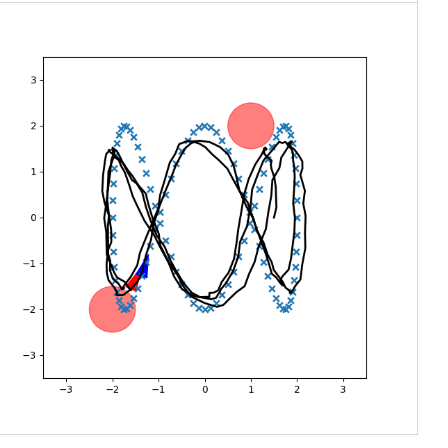
\includegraphics[width=0.6\textwidth]{CEC.png}
    \caption{Trajectory followed by the agent using CEC controller}
    \label{fig:cec}
\end{figure}
\subsection{Generalized Policy Iteration}
The trends in the tuning of the hyperparameters of GPI are similar to that of CEC. The hyperparameters used are:
\begin{align*}
    \gamma &= 0.7 \\
    T &= 10 \\
    Q &= \begin{bmatrix}
        3.5 & 0  \\
        0 & 7 
    \end{bmatrix} \\
    R &= \begin{bmatrix}
        8 & 0  \\
        0 & 0.1
    \end{bmatrix} \\
    q &= 7000
\end{align*}
\subsection{Comparison}
Although GPI controller gave better trajectory but it still really high computation time when compared to CEC controller.
Since, we assigned a cost function for the obstacle avoidance in the GPI controller, it was able to avoid the obstacle more effectively than the CEC controller, where it had solve an optimization problem to avoid the obstacle by fitting the constraints.

\end{document}
